\documentclass[border=10pt]{standalone}
\usepackage{pgfplots}
\usepgfplotslibrary{colormaps}
\pgfplotsset{compat=1.18}

\begin{document}
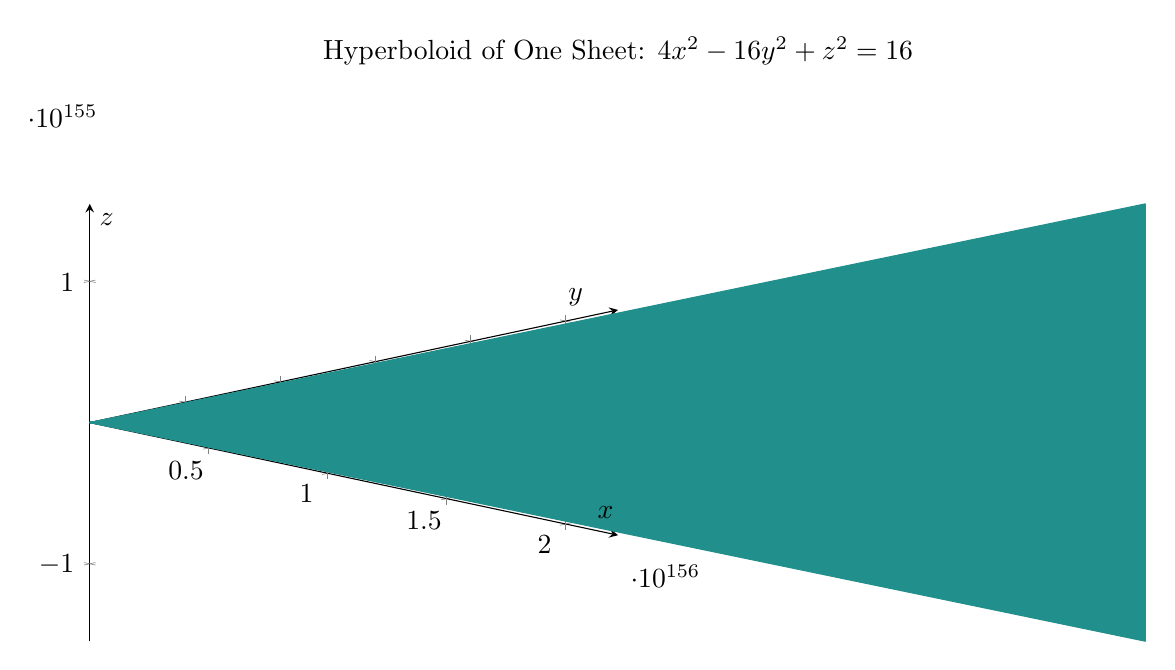
\begin{tikzpicture}
\begin{axis}[
    view={45}{20},
    xlabel=$x$,
    ylabel=$y$,
    zlabel=$z$,
    title={Hyperboloid of One Sheet: $4x^2 - 16y^2 + z^2 = 16$},
    colormap/viridis,
    width=15cm,
    height=10cm,
    axis lines=center,
    enlargelimits=false,
    samples=30,
    domain=-2:2,
    y domain=0:360,
]
\addplot3[surf, shader=flat corner] (
    {2*cos(x)*cosh(y)},
    {sinh(y)},
    {4*sin(x)*cosh(y)}
);
\end{axis}
\end{tikzpicture}
\end{document}
